% ----------------------------- NO NEED TO WORRY ABOUT WHAT IS BELOW ---------------------------
%--------------------
% Packages
% -------------------
\documentclass[a4paper]{article}
\usepackage[utf8x]{inputenc}
\usepackage[T1]{fontenc}
\usepackage[pdftex]{graphicx} % Required for including pictures
\usepackage[pdftex,linkcolor=black,pdfborder={0 0 0}]{hyperref} % Format links for pdf
\usepackage{calc} % To reset the counter in the document after title page
\usepackage{enumitem} % Includes lists
\frenchspacing % No double spacing between sentences
\linespread{1.2} % Set linespace
\usepackage[a4paper, lmargin=0.1\paperwidth, rmargin=0.1\paperwidth, tmargin=0.1111\paperheight, bmargin=0.1111\paperheight]{geometry} %margins
\usepackage[all]{nowidow} % Tries to remove widows
\usepackage[protrusion=true,expansion=true]{microtype} % Improves typography, load after fontpackage is selected
\usepackage{pdfpages}
\usepackage[title]{appendix}
\usepackage{listings}
\usepackage{color}
\usepackage{multicol}
\usepackage{amsmath} 
\usepackage{colonequals}
\usepackage{amssymb}
\usepackage{graphicx} 
\usepackage{subfig}
\usepackage{float}
\definecolor{mygreen}{rgb}{0,0.6,0}
\definecolor{mygray}{rgb}{0.5,0.5,0.5}
\definecolor{mymauve}{rgb}{0.58,0,0.82}
\lstset{ 
  backgroundcolor=\color{white},   % choose the background color; you must add \usepackage{color} or \usepackage{xcolor}; should come as last argument
  basicstyle=\footnotesize,        % the size of the fonts that are used for the code
  breakatwhitespace=false,         % sets if automatic breaks should only happen at whitespace
  breaklines=true,                 % sets automatic line breaking
  captionpos=b,                    % sets the caption-position to bottom
  commentstyle=\color{mygreen},    % comment style
  deletekeywords={...},            % if you want to delete keywords from the given language
  escapeinside={\%*}{*)},          % if you want to add LaTeX within your code
  extendedchars=true,              % lets you use non-ASCII characters; for 8-bits encodings only, does not work with UTF-8
  frame=single,	                   % adds a frame around the code
  keepspaces=true,                 % keeps spaces in text, useful for keeping indentation of code (possibly needs columns=flexible)
  keywordstyle=\color{blue},       % keyword style
  language=python,                 % the language of the code
  morekeywords={*,...},            % if you want to add more keywords to the set
  numbers=left,                    % where to put the line-numbers; possible values are (none, left, right)
  numbersep=5pt,                   % how far the line-numbers are from the code
  numberstyle=\tiny\color{mygray}, % the style that is used for the line-numbers
  rulecolor=\color{black},         % if not set, the frame-color may be changed on line-breaks within not-black text (e.g. comments (green here))
  showspaces=false,                % show spaces everywhere adding particular underscores; it overrides 'showstringspaces'
  showstringspaces=false,          % underline spaces within strings only
  showtabs=false,                  % show tabs within strings adding particular underscores
  stepnumber=2,                    % the step between two line-numbers. If it's 1, each line will be numbered
  stringstyle=\color{mymauve},     % string literal style
  tabsize=2,	                   % sets default tabsize to 2 spaces
  title=\lstname                   % show the filename of files included with \lstinputlisting; also try caption instead of title
}
\usepackage{etoolbox}
\patchcmd{\maketitle}{\@fnsymbol}{\@alph}{}{}  % Footnote numbers from symbols to small letters
\usepackage{svg}
\DeclareSymbolFont{symbolsC}{U}{pxsyc}{m}{n}
\DeclareMathSymbol{\coloneqq}{\mathrel}{symbolsC}{"42}
\usepackage{algorithm}
\usepackage[noend]{algpseudocode}
% ----------------------------- NO NEED TO WORRY ABOUT WHAT IS ABOVE ---------------------------

%-----------------------
% Title, Authors
%-----------------------
\title{\vspace{-3.5cm} %
  Spectral Clustering and Network Analysis \\
  of the Cryptocurrency Market \\ \vspace{.2cm}
  \large Replication of  Kwapień et al.\cite{kawpien}}
\date{May 4, 2017}
\author{Nick Eterovic\thanks{neterovi@andrew.cmu.edu, Pittsburgh Campus} \quad \quad Andrew Previc\thanks{aprevic@andrew.cmu.edu, Pittsburgh Campus} \quad  \quad 
		Eloy Lanau-Rosello\thanks{elanauro@andrew.cmu.edu, Pittsburgh Campus} \quad \quad Justin Skillman\thanks{jskillma@andrew.cmu.edu, Pittsburgh Campus}}

%-----------------------
% Begin document
%-----------------------
\begin{document} 
\maketitle
\tableofcontents
\newpage
\begin{multicols}{2}

%-----------------------
% Begin main section
%-----------------------
\section{Introduction}\label{intro} % Section Headings
Our project replicates Kwapień et al.'s\cite{kawpien} network analysis of the foreign exchange (FX) market and applies similar statistical analysis to the cryptocurrency market. Kwapień et al. clusters the time series data of 63 currencies and assets using a filtered correlation matrix method and produces both fixed-time and time-dependent eigenspectra graphs. Using the eigenspectra graphs, the authors identify those currencies heavily ``coupled'' with the FX market as a whole and how those coupling relationships change over time. We subsequently apply a similar clustering method to 18 of the most heavily traded cryptocurrencies and produce both fixed-time and time-dependent eigenspectra graphs. In addition to the filtered correlation method used by Kwapień et al., we also implement spectral clustering to analyze the data. In Section \ref{spectral}, we introduce spectral clustering and discuss its superiority over traditional clustering methods such as k-means and single linkage when analyzing time series data. In Section \ref{crypto} we assess the significant ways in which the cryptocurrency market differs from the FX market and note interesting observations in the data and suggest possible explanations in real world events. In Section \ref{further} we discuss avenues for future research given our findings and questions generated as a result.

\section{Replication of Kwapień et al.}\label{kwapien}

\subsection{Data and methods}
Kwapień et al. analyzed a total of 63 assets: 60 currencies and 3 precious metals. Gold, silver and platinum were included in the analysis given the historical use of these precious metals as a store of wealth during periods of high inflation, economic uncertainty, and currency market crises. Another reason for their inclusion is that the FX market lacks an independent reference asset. Comparing two currencies denominated in gold, for example, avoids the problem of introducing hidden dependencies by using a third currency. The 60 currencies were chosen in descending order by trade volume. The five most significant (USD, EUR, JPY, GBP, AUD) account for 82\% of global trade volume, after which trade volume diminishes according to a power law. Five emerging market currencies (ZMW, PAB, HRK, EEK, BSD) were pegged to the US dollar for the entire data set - their constant time series were omitted to calculate complete cross-currency correlations. 
The data set spans 9.5 years from January 1, 1999 to June 30, 2008. As the global currency system is decentralized, the forex market remains open 24 hours per day, 7 days per week. However, liquidity rapidly declines from 5pm Friday to 5pm Sunday. Although the time period consists of 3468 trading days, we omit weekends during which the lack of trading volume adversely affects the accuracy of daily data. The resulting data consists of $M=58$ USD-denominated exchange rates over $N=2394$ trading days. Assuming an absence of triangular arbitrage, we have $58(58-1) = 3306$ time series at our disposal.
Selecting a base currency B yields a $N \times M$ data matrix $X_B$ , in which each column corresponds to the log-return time series of a $B$-denominated exchange rate. From $X_B$ we calculate its $M \times M$ correlation matrix $C_B = X_B^TX_B/N$. The market global correlation structure, viewed from the perspective of base currency B, can be quantified from the eigenvalue spectra of $C_B$. In particular, let $\lambda_B^{max}$ denote the largest eigenvalue of $C_B$. Comparison of $\lambda_B^{max}$ across different base currencies, see Figure \ref{fig:fxeigenspectra} (from Kwapień et al.), indicates the dependency of a given currency's movement with that of the broader FX market.
\begin{figure}[H]
\centering
    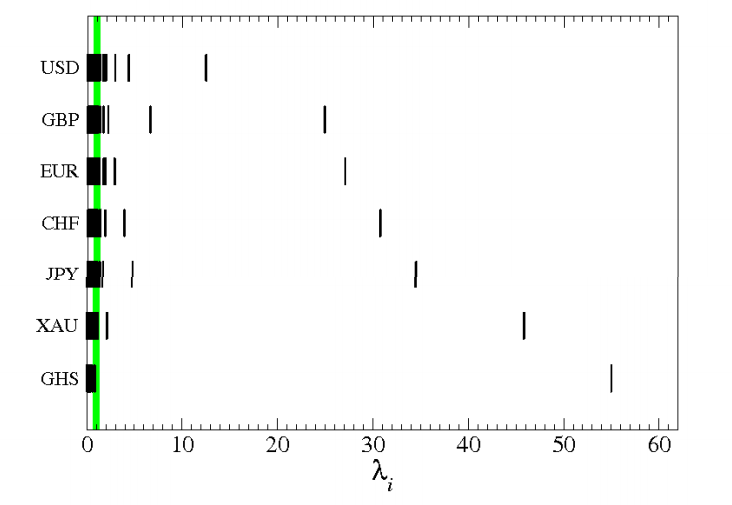
\includegraphics[totalheight=5cm]{BaseEigenvalues.PNG}
    \caption{Eigenvalue spectra for exemplary base currencies. The United States dollar (USD) and Ghanaian Cedi (GHS) have the smallest and largest maximum eigenvalues, respectively, indicating their roles as central (market-shaping) and peripheral (market-influenced) currencies.}	
    \label{fig:fxeigenspectra}
\end{figure}

\subsection{Dissimilarity measures and minimum spanning trees.}\label{dist}
Studying the dependency structure in $C_B$ is made accessible by defining an associated dissimilarity matrix $D_B$ with the formula:
$$D_B(i,j)=\sqrt{2(1-C_B(i, j))}$$
The entries of $D_B$ lie in $(0, 2)$. Values near $0$, $\sqrt{2}$, and $2$ correspond to positively correlated, uncorrelated, and negatively correlated time series, respectively.
Kwapień et al. use the minimum spanning tree (MST) to visualize dependencies. An MST sequentially connects closest nodes with respect to $D_B$ but in such a way that each pair of nodes is connected by a single path. The result is a distance matrix $D_B^{MST}$ and only $N-1$ (rather than $N(N-1)/2$) edges connecting $N$ nodes. The appeal of the MST is in its sparsity - with so few edges, key nodes can easily be identified by a high number of neighboring nodes (degree). Moreover, the MST can be visualized in a 2D plane with no intersecting edges, see Figure \ref{fig:mstfx} (from Kwapień et al.).
\begin{figure}[H]
\centering
    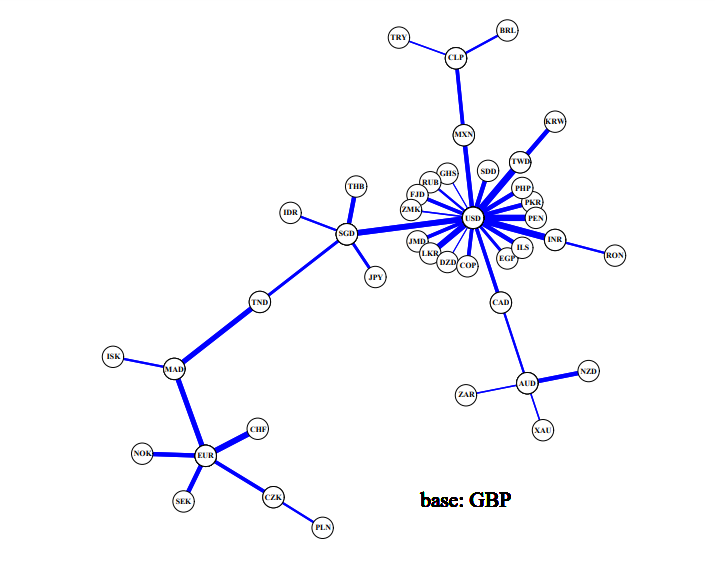
\includegraphics[totalheight=6cm]{MSTfx.PNG}
    \caption{Minimum spanning tree}	
    \label{fig:mstfx}
\end{figure}
Changes in the global currency system with time can be characterized by the changing eigenvalue spectra, see Figure \ref{fig:timefx} (from Kwapień et al.), - an increasing maximum eigenvalue quantifies a currency's role transitioning from central to peripheral  
\begin{figure}[H]
\centering
    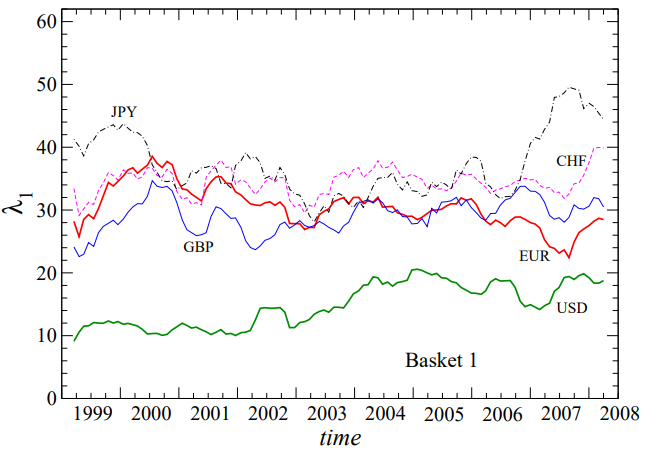
\includegraphics[totalheight=5cm]{EigenvalueTemporal.PNG}
    \caption{Time-evolution of maximum eigenvalues}	
    \label{fig:timefx}
\end{figure}

\subsection{Observations}
In replicating Kwapień et al., we observe the relationship between various fiat legacy currencies in Europe such as the Drachma, the Lira, the Cypriot Pound, and the Euro. The Swiss Franc, until 2015, for example, had been pegged to the Euro and we thus see the strength of that pegged relationship in our correlation heat matrix. We also see the strong correlation between silver and gold, which again is to be expected given the similar price dynamics of precious metals.
The Hong Kong Dollar (HKD/USD) exhibits little to no correlation with other exchange rates, explained by the fact that HKD is pegged to the USD. The peg causes HKD to in effect serve as a base currency in all exchange rate relationships and thus eliminate any particular relationship HKD might have with a non-USD pegged currency.
In our first cluster diagram, we again see the clustering relationship among silver, gold and platinum, all precious metals with similar price fundamentals. The other currencies are related either by geographical region or, specifically in the case of Europe, as legacy currencies pegged to the Euro prior to their dissolution. An interesting observation is the relationship between the Jordan Dinar and the Kuwaiti Dinar, likely due to the economic and regional similarities of both countries, as well as, the fact that the Jordan Dinar is pegged to the US Dollar while the Kuwaiti Dinar was pegged to the US Dollar between 2003 and 2007.
Our Spectral Clustering and Spectral Clustering with Connected Subgraph Analyses show the Kuwaiti Dinar's connection to a number of other currencies, which is likely due to the fact that the Kuwaiti Dinar is pegged to a basket of currencies, as well as the fact that, as a major oil exporter, Kuwait's own GDP is dependent on the economic growth and health of a number of oil-consuming countries.
Assessing the largest eigenvalue for the USD over time, we observe a diminishing central role -although still significant - relative to the system. While the USD remains a dominant currency globally, it is clearly no longer the sole global reserve currenc. In particular, the Euro and Chinese Yuan have gained popularity as alternative stores of investment value over the time period.

\section{Spectral clustering}\label{spectral}
Many of the clustering techniques we have learned throughout the ML sequence in the MSCF program only work well for convex or ``blob'' type data. When the data is non-convex, the performance of these techniques decreases substantially. This happens because these methods use elliptical metrics to form the clustered groups. Following the canonical example of concentric crescents shown in Figure \ref{fig:nonconvex} we can see that k-means where $k=3$ would result in a clearly incorrect clustering. This is a well known problem and much work has been done on methods that overcome this issue such as hierarchical clustering using single-linkages. Spectral clustering has become one of the most popular methods to cluster non-convex data.
\begin{figure}[H]
\centering
    
\includegraphics[totalheight=3cm]{nonconvex_sets.png}
    \caption{K-means on non-convex data}
    \label{fig:nonconvex}
\end{figure}
As noted in Wang and Zhang (2005) \cite{spectraltime}, time series are not amenable to being clustered using traditional methods such as k-means. They can be of varying length depending on the number of observations and are often very high dimensional. The authors have proposed spectral clustering as a means to get past these problems. Of the most important reasons to use spectral clustering in the case of time series is that the dimensionality does not affect the computational costs of running the algorithm. When one has an appropriate similarity measure or distance matrix, this can be fed into the algorithm without extra computational burden for even very high dimensional time series. For example if you had hourly time series for ten currencies over a week versus over a decade, given that one has a distance matrix for both, the spectral clustering takes the same amount of time in either case. Different methods can be used to compute the distance matrix, in our case we will use the same as for Minimum Spanning Trees. Below we guide the reader through an introduction to spectral clustering starting from the basic building blocks progressing to interpretations of the algorithm's output.

\subsection{Basics}
Given a positive similarity metric $s_{ij} \coloneqq \text{similarity}(x_i, x_j) \geq 0$  between points in some set, $\{x_1,x_2,..., x_N \}$, clustering can be thought of as attempting to form groups where the in-group similarity metrics are high and the out-group similarity is low. An often used similarity metric is that of the radial basis function kernel (RBF). There is an entire sub-field of mathematics devoted to studying problems of this type, graph theory. Spectral clustering uses much of the methodology from this area. 

The basic building blocks are as follows, we represent vertices (or nodes) as belonging to the set $V = \{v_1, ..., v_N \}$. Let $E$ be the set of edges or connections between vertices, where each edge is weighted with some similarity metric $w_{ij} = s_{ij}  \forall \hspace{0.1cm} i \neq j$, $w_{ii}$ is often taken to be zero though that ultimately won't change the results of the algorithm at all. $G = (V, E)$ is then a fully defined graph. The weights form a weighted-adjacency matrix $W = (w_{ij})_{i,j=1,...N}$. In our case the graph is undirected, meaning connections are independent of direction being traveled between nodes. This means that $w_{ij} = w_{ji}$, the adjacency matrix is symmetric. The degree of a vertex measures how strong the connections are that exist between it and other vertices,
$$
d_i = \sum_{j=1}^N w_{ij}.
$$
Using the set of $\{d_1,..,d_N\}$ we form a diagonal matrix. This matrix, $D$, is the degree matrix of size $N \times N$. Please note that we use $D$ to represent the distance matrix later in the document but in this section we use it to represent the degree matrix. 
\begin{figure}[H]
\centering
    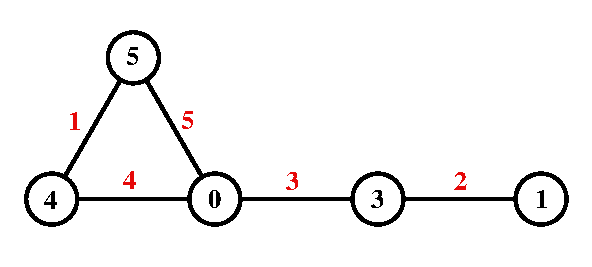
\includegraphics[totalheight=2.5cm]{graph.pdf}
    \caption{Undirected Weighted Graph}
    \label{fig:graph1}
\end{figure}
Using the example in Figure \ref{fig:graph1} where we assume vertex 2 (not shown) has no connections, we would have the following for $W$ and $D$. Please note we use zero-based indexing here.
$$
W = 
\begin{pmatrix}
0 & 0 & 0 & 3 & 4 & 5 \\
0 & 0 & 0 & 2 & 0 & 0 \\
0 & 0 & 0 & 0 & 0 & 0 \\
3 & 2 & 0 & 0 & 0 & 0 \\
4 & 0 & 0 & 0 & 0 & 1 \\
5 & 0 & 0 & 0 & 1 & 0 \\
\end{pmatrix}
$$
$$
D = 
\begin{pmatrix}
12 & 0 & 0 & 0 & 0 & 0 \\
0 & 2 & 0 & 0 & 0 & 0 \\
0 & 0 & 0 & 0 & 0 & 0 \\
0 & 0 & 0 & 5 & 0 & 0 \\
0 & 0 & 0 & 0 & 5 & 0 \\
0 & 0 & 0 & 0 & 0 & 6 \\
\end{pmatrix}
$$
\newline
The final basic building block one should know is the notion of connected components. If $A \subseteq V$, $A$ is said to be a connected component of $G$ if any two vertices $v_i, v_j \in A$ can be connected such that all intermediate vertices are also in $A$.

\subsection{Graph Laplacians}
The Laplacian matrix is an extremely useful tool that can be used to find many properties of a graph. It is defined as,
$$
L = D - W.
$$
As noted above one can see that it won't matter what you make the self-to-self weighting for the vertices. Any self weighting will result in the exact same $L$.
\newline
\textbf{Properties of $L$}
\begin{enumerate}
\item $L$ is symmetric and positive semi-definite
\item All of the row and column sums of $L$ equal 0
\item The smallest eigenvalue of $L$ is zero with eigenvector $v = (1, 1, ..., 1)$
\item $L$ has $N$ non-negative eigenvalues 0 $=\lambda_1 \leq \lambda_2 \leq ... \leq \lambda_N$
\item $\forall  f \in \mathbb{R}^N$,   \text{(the proof of this can be found in \cite{spectral})}
$
f'Lf = \frac{1}{2} \sum_{i,j = 1}^N w_{ij}(f_i - f_j)^2. 
$
\end{enumerate}
One of the most interesting and useful properties of $L$ is that the the number of connected components in $G$ is equal to the algebraic multiplicity of eigenvalue 0. This is also equal to the dimension of the nullspace of $L$. To show this is true imagine a case where there is only one connected component, the whole graph. If the eigenvector pertaining to the eigenvalue 0 is $f$ then from the properties above we have,
\begin{equation}\label{eq}
0 = f' L f = \sum_{i,j=1}^N w_{ij}(f_i - f_j)^2.
\end{equation}
Every term in the summation is non negative as the second term is squared and the weights in our graph are non-negative. This means that for the equality to hold every $w_{ij}(f_i - f_j)^2$ must equal zero. This graph is connected so all $w_{ij} > 0 \hspace{0.1cm} \forall \hspace{0.1cm} i \neq j$. This means that $f_i=f_j$, thus $f$ needs to be a vector where every element is equal. After normalizing, $f$ is then $(1, 1, ..., 1)$ or the unit vector. A similar argument holds for a graph with $n$ connected components. The matrices $W$ and thus $L$ will now be block diagonal if we order them according to which connected component they belong to. We call each block $L^i$. Equation \ref{eq} still needs to hold and knowing that each block $L^i$ is a connected component it has $f^i = (1, 1, ..., 1)$ thus $f$ for the entire $L$ is this vector padded with zeros where the other blocks are. There will precisely $n$ of these vectors. For example, if each block was size $2 \times 2$ and there were $n=3$ blocks, meaning $N=6$, the 3 normalized eigenvectors pertaining to the eigenvalue zero would look like, $v_1 = (1, 1, 0, 0, 0, 0)$, $v_2 = (0 ,0, 1, 1, 0, 0)$, and $v_3 = (0, 0, 0, 0, 1, 1)$. In reality we will not observe completely disconnected sub-graphs but some perturbation of $L$. This perturbation \textit{will not} substantially affect the resultant vectors. As show in Sun and Stewart (1990) \cite{perturb} the stability of the eigenvectors is determined by the eigengap betwen $\lambda_k$ and $\lambda_{k+1}$. 
In a number of experiments run in Ng et al. (2001) \cite{ng}, this eigengap is large for most any reasonable perturbation. As such they provide a reasonable matrix (when stacked) on which to cluster the rows. We discuss this in detail later in this section.
\end{multicols}

\subsection{Algorithm}
\begin{algorithm}[H]
\caption{Spectral Clustering}\label{spectralalg}
\begin{algorithmic}[H]
\State \textbf{\textit{Input:}} Weighted adjacency matrix $W \in \mathbb{R}^{N \times N}$, number of clusters $k$
\State Compute degree matrix $D$
\State $L \gets D - W$ 
\State Compute first $k$ eigenvectors $v_1, ..., v_k$  of $L$ and stack them into $X \in \mathbb{R}^{N \times k}$
\State $y_i \gets$ normalized ith row of $X \quad$   (note: $y_i \in \mathbb{R}^{k}$)
\State Cluster $(y_i)_{i=1,...,n}$ into clusters $C_1, ..., C_k$ using k-means
\State \textbf{\textit{Output:}} Clusters $A_1,...,A_k$ where $A_i = \{j | y_j \in C_i \}$
\end{algorithmic}
\end{algorithm}

\begin{multicols}{2}
\subsection{Intuition and interpretation}
\begin{figure}[H]
    \centering
    \subfloat[Non-convex original data]{{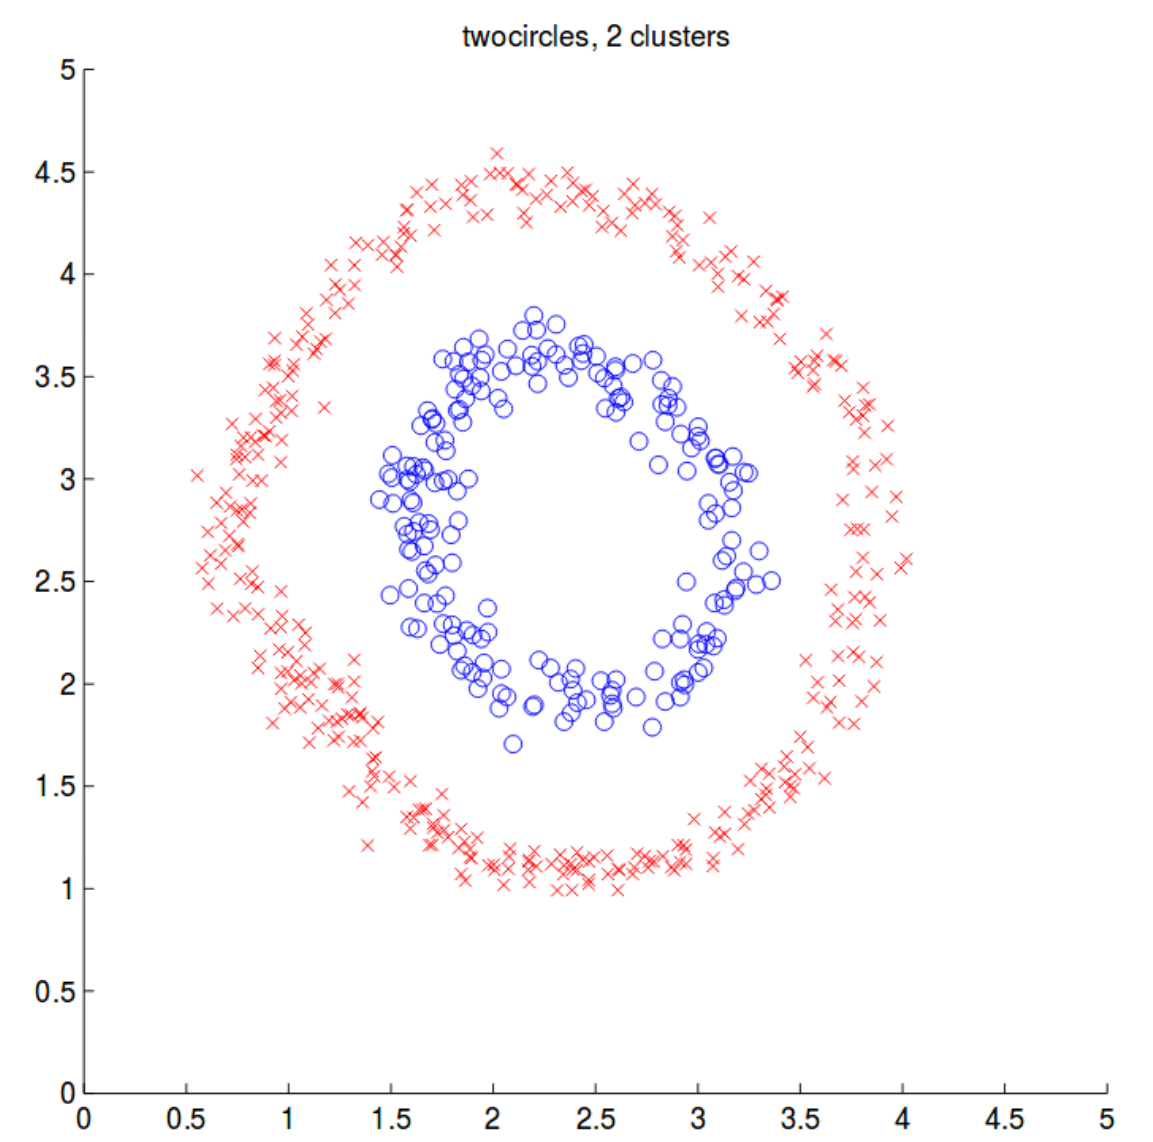
\includegraphics[width=3.5cm]{two_circles.png} }}
    \quad
    \subfloat[$y_1$ and $y_2$ (rows in $X$)]{{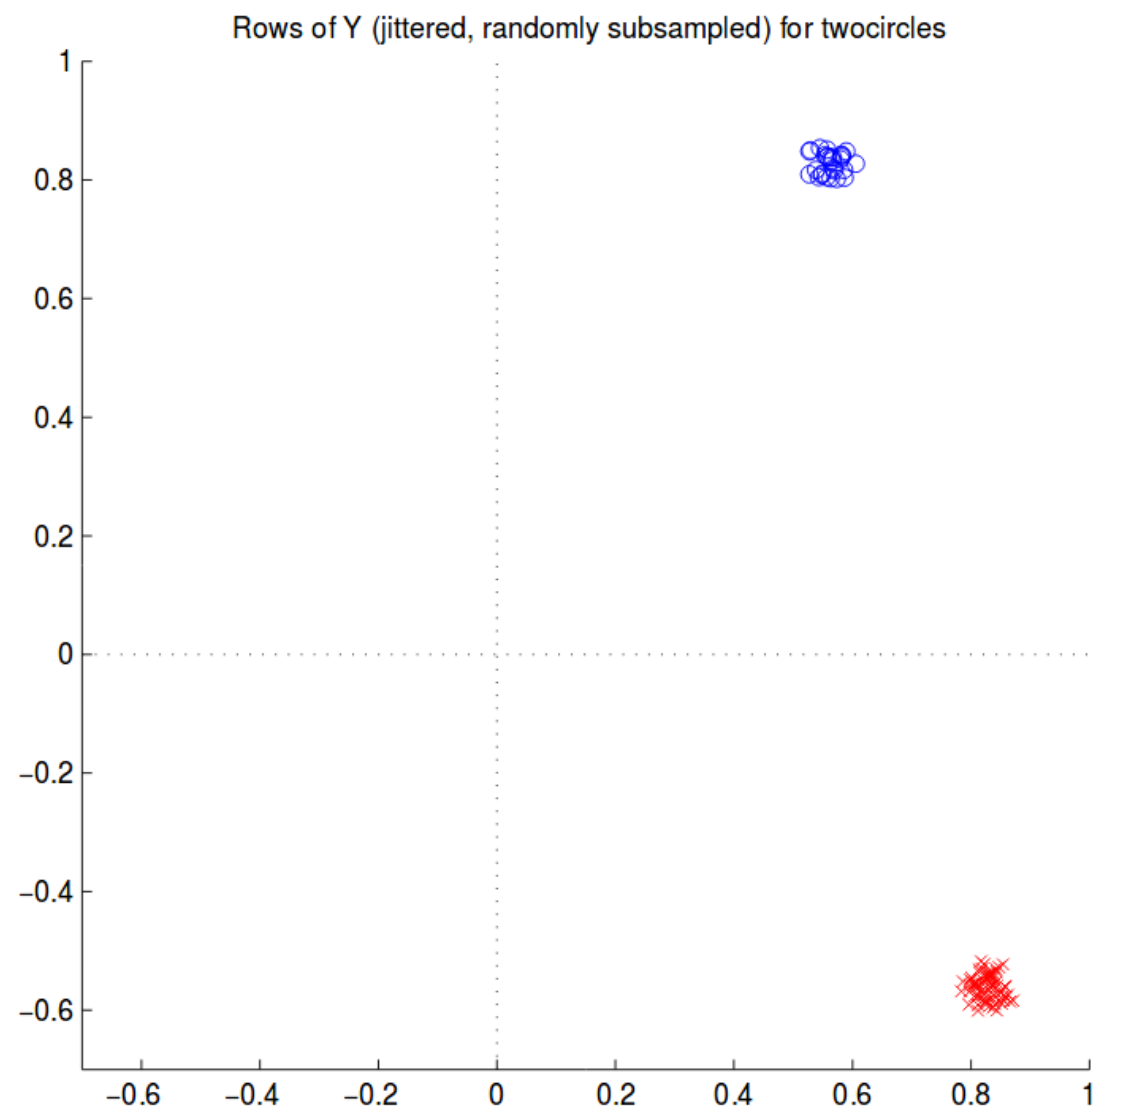
\includegraphics[width=3.5cm]{rowsy.png} }}
    \caption{Why k-means works on $y_i$'s}%
    \label{fig:yrowsex}%
\end{figure}
After reading Algorithm \ref{spectralalg}, it may not seem obvious why spectral clustering works at all. Namely, one may wonder why we use k-means after all of the fuss about it performing so poorly for time series. The reason for this seeming inconsistency is that in using the algorithm above we transform into a space that is extremely amenable to being clustered using traditional methods. The choice of k-means is somewhat arbitrary and even simple methods like linear classifiers work well on the rows $y_i$. As can be seen in Figure \ref{fig:yrowsex} from \cite{ng} separation of the $y_i$ vectors in the $k=2$ dimensional space is trivial. One should also be aware that the smallest eigenvalues will not be identically zero but are interpreted as such when small enough, this happens because we are not in the ideal ``noiseless'' case.
Care should also be taken in choosing $k$, the number of clusters the algorithm will group $y_i$'s into. Some authors have chosen $k$ to be the $k$-th eigenvalue directly prior to a jump in the eigenvalues (when sorted). This method has been controversial as there is little theoretical backing for doing so and is heavily dependent on specific qualities of the data. Zelnik-Manor and Perona (2005) propose a self-tuning process that chooses $k$ from the eigenvectors by maximizing sparseness in the matrix of $k$ eigenvectors. At the most basic level one could use qualitative knowledge, in our case about the geographic or legal aspects of the currency market that would lead to some specific number of clusters.

\section{Application to cryptocurrency market}\label{crypto}

\subsection{Data}
For our analysis with cryptocurrencies we use hourly data\cite{cryptodownload} for 18 cryptocurrencies plus USD. We decided to obtain all of these pairs from one exchange, Poloniex\cite{poloniex}. Cryptocurrency prices vary strongly from one exchange to another depending on how easy it is to trade them. Examples of difficulties would be capital restrictions, commissions and the number of currency pairs they trade against. We decided to use only data from one exchange as a way to hedge our time series correlation from these changes. While Poloniex is only the 29\textsuperscript{th} largest exchange by trading volume\cite{coinmarketcap}, we chose it because it is based in the US, has low capital restrictions, trades numerous cryptocurrency pairs and freely provides historical hourly quotes.
We decided to carry out this analysis with hourly prices because, given the recent introduction of some cryptocurrencies, we did not have sufficient observations for daily price analysis. For example, IOTA was launched on June 13\textsuperscript{th}, 2017, so we could only obtain 172 daily observations. Increasing our frequency to hourly we obtained between 5,242 and 7,167 observations for each of the pairs with data from July 1\textsuperscript{st}, 2017 to April 26\textsuperscript{th}, 2018.

\subsection{Methods and initial observations}
We start our analysis following the approach used for traditional currencies. We consider BTC to be the equivalent of USD but in the cryptocurrency market because it is the most traded and valuable cryptocurrency and because it is the most common asset necessary to buy other cryptocurrencies, a similar role played by USD in the global FX market.

Two of the most important aspects of cryptocurrency market dynamics are bridge currencies and use cases. Bridge currencies exist due to the fact that many cryptocurrencies cannot be acquired with fiat currencies, only with other crypto currencies known as “bridges”. To access more niche or use-specific crypto-currencies, investors must first exchange dollars or euros, etc. into more liquid bridge currencies, notably Bitcoin (BTC), Ethereum (ETH), Bitcoin Cash (BCH) and Litecoin (LTC). An expected observation confirmed in our data is the importance of the bridge currencies in the broader cryptocurrency market as indicated by lower max eigenvalues in our eigenspectra analysis.

Use cases refer to the differentiated uses and market segmentation of the individual cryptocurrencies. Cryptocurrencies are often associated with specific market segments, services, or products. BeeToken (BEE), for example, is a cryptocurrency formed solely to process AirBnb transactions. Investors may take a specific position in a niche crypto given a belief in the crypto’s ability to take market share from other cryptocurrencies. Such motivation is different from a desire to invest in the entire cryptocurrency market (often guided by mainstream speculation), and thus, results in differentiated price dynamics.

\subsubsection{Eigenspectra of CM for different base currencies}
Figure \ref{fig:eigenspectra} shows the cryptocurrency eigenspectra.
\end{multicols}
\begin{figure}[H]
\centering
    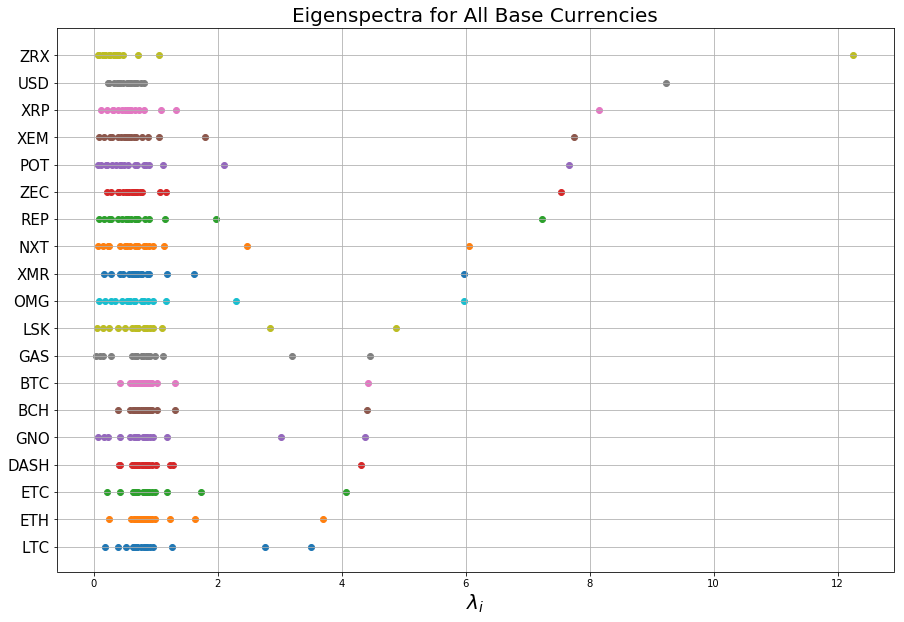
\includegraphics[totalheight=8cm]{Eigenspectra.png}
    \caption{Eigenvalue spectra of the correlation matrices calculated per each cryptocurrency (and USD) as base}	
    \label{fig:eigenspectra}
\end{figure}

\begin{multicols}{2}

An interesting observation is how large the max eigenvalue is for Ripple (XRP). 0x (ZRX) has the highest max eigenvalue but is also one of the smallest cryptocurrencies examined by market cap (\$689 million vs. \$154 billion for BTC). It further differentiates itself to Bitcoin and other bridge currencies by its unique technology, which offers off-chain ordering books with on-chain settlements or transactions on the Ethereum network so its preference among certain crypto enthusiasts might explain its differentiated time series. Ripple, on the other hand, has a market cap of \$34 billion and yet has been one of the least correlated cryptocurrencies with the broader cryptocurrency market historically. This has interesting hedge implications for serious cryptocurrency investors willing to selectively parse cryptocurrency as an asset class. 

The low max eigenvalues of the aforementioned bridge currencies make sense for the reasons given above. That being said, there is a less clear explanation as to why Litecoin and Dash would have a significantly lower max eigenvalue than other bridge currencies, given the clear market preference for Bitcoin as a crypto investment (LTC market cap \$8 billion vs. \$154 billion BTC market cap). That being said, a likely cause is the influx of speculative capital beginning August 2017 as we discuss in further detail below.

Another interesting observation from the eigenspectra analysis is the relatively large max eigenvalue of USD in relation to the max eigenvalues of the other cryptocurrencies. The observation indicates that the US dollar’s time series is unbundled from that of other cryptocurrencies. This is an interesting finding considering the US dollar’s central role in the eigenspectra for fiat currencies as highlighted above. Given the observed divergence in precious metal prices with those of the crypto market in general over the 2011-present period, we would also anticipate a similar unbundled relationship with the crypto market as well. 

\subsubsection{Temporal stability of the market structure}
Figure \ref{fig:lambda1_time} show the value of the highest eigenvalue per each base over time computed as a 60-day rolling average.
\end{multicols}
\begin{figure}[H]
\centering
    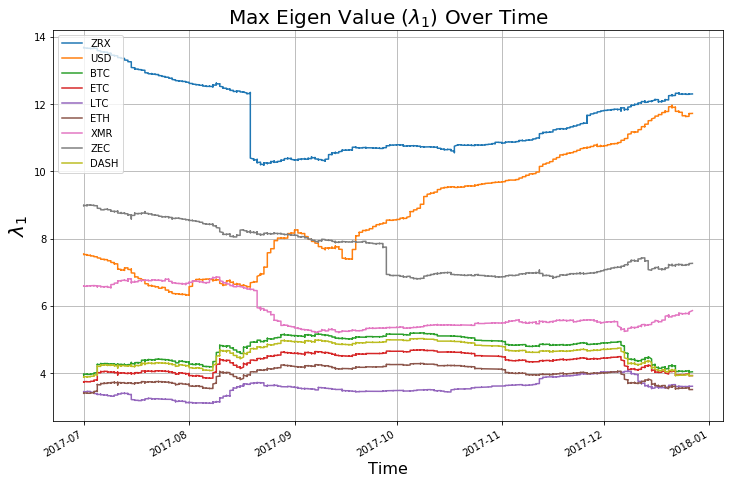
\includegraphics[totalheight=8cm]{lambda1_time.png}
    \caption{Max eigenvalue value over time for different bases}
    \label{fig:lambda1_time}
\end{figure}
\begin{multicols}{2}

In analyzing the largest eigenvalues over time, we see a general convergence across all crypto currencies between August 2017 and January 2018. The convergence of max eigenvalues indicates the cryptocurrency market becoming either more tightly bundled or equally unbundled in terms of similarity of time series. This convergence corresponds with the influx of speculative money into the market as the rise of Bitcoin and other cryptocurrencies became better known to the general public. The influx of speculative money was largely undifferentiated with regards to a specific cryptocurrency given the rather unsophisticated nature of speculative investors to distinguish one currency from another. The sharp fall in the largest eigenvalue for Monero (XMR) in the month of August, for example, corresponds with the rise in the cryptocurrency’s price from \$50 to \$100 over that same period. Even more drastic is the fall in value of the largest eigenvalue for Dash (DASH) in late August, which corresponds with the currency having hit an all-time price high on news of a new Blockchain Research Lab partnership between Dash and Arizona State University. 

\subsubsection{Cluster structure of the cryptocurrency market}
To study the cluster structure of the cryptocurrency market we use the two methods outlined in \cite{kawpien} and spectral clustering as a new method to try to better cluster the data. We chose to use USD, BTC, ETH and LTC as the base currencies for our clustering. The first three because of their role as a medium to buy other currencies and LTC because is the one with the smallest max-eigenvalue.

The network structure found by thresholding the correlation matrix is shown in Figure \ref{fig:Cthres_crypto}.
%\end{multicols}
\begin{figure}[H]
\centering
    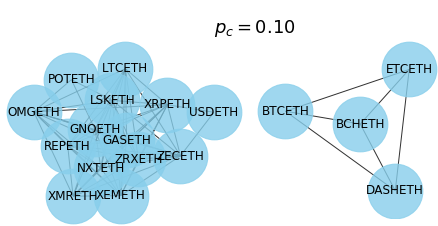
\includegraphics[totalheight=4.2cm]{Cthres_crypt.png}
    \caption{Clustering obtained by thresholding the correlation matrix obtained using ETH as the base currency}
    \label{fig:Cthres_crypto}
\end{figure}
%\begin{multicols}{2}
In the Thresholding $C$ cluster analysis with correlation as the distance measure and BTC as the base, we see edges between and among the largest cryptocurrencies by market cap with smaller cryptocurrencies by market cap remaining unconnected. With USD as the base and using a correlation of .7 as a threshold, the only edges that remain are those connecting bridge currencies, again highlighting the similarities of the price dynamics of ETH, BTC, BCH and LTC.With ETH as a base, we observe similar bridge currency clustering, however, also with the inclusion of DASH, which is an interesting observation but likely explained by the high historical correlation between DASH and ETH.

Using the metric $D_B(i,j)$ defined in Subsection \ref{dist} we compute the MST of our data. It is plotted in Figure \ref{fig:MST_crypto}.
\end{multicols}
\begin{figure}[H]
\centering
    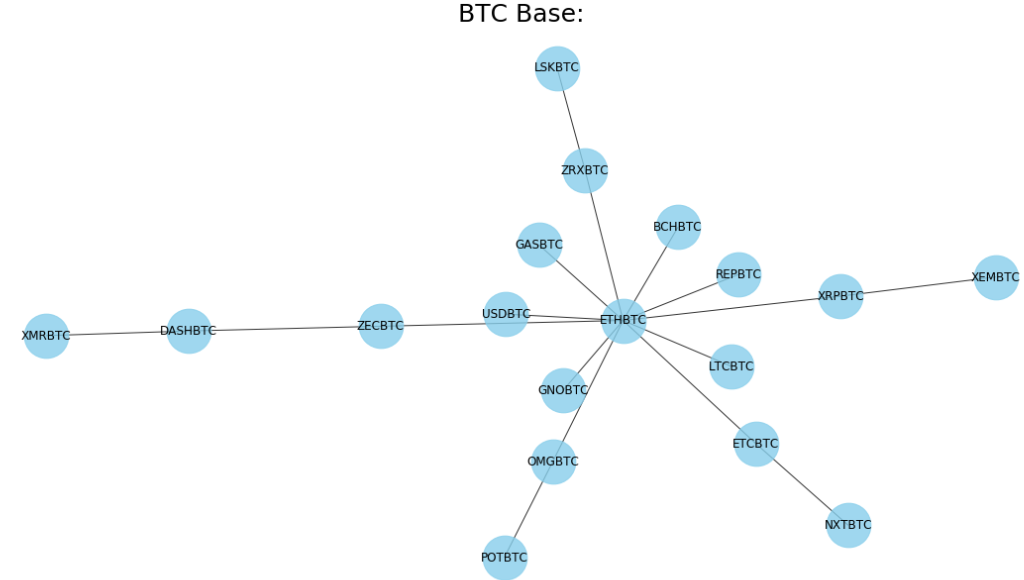
\includegraphics[totalheight=6.5cm]{MST_cropped.PNG}
    \caption{Clustering representation obtained using MST of our cryptocurrencies using BTC as the base}
    \label{fig:MST_crypto}
\end{figure}
\begin{multicols}{2}
From the MST representation we see the centrality of ETH. The explanation could be because it may be linked to plenty of altcoins that can only be bought using ETH.


\paragraph{Spectral Clustering}
We perform Spectral Clustering using the same distance metric, defined in Subsection \ref{dist}. The results are in Figure \ref{fig:spectralclust_Crypto}.
The results found using Spectral Clustering are the following.

\end{multicols}
\begin{figure}[H]
\centering
    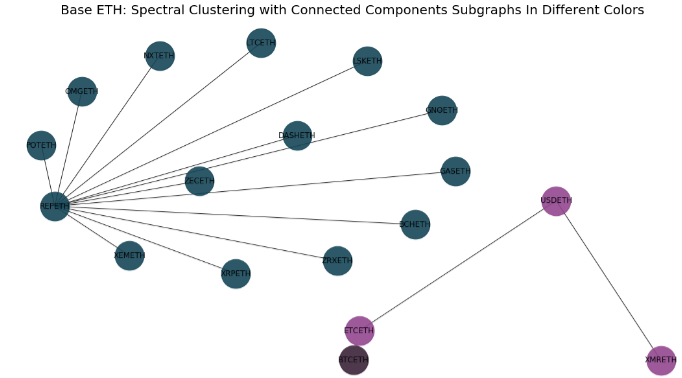
\includegraphics[totalheight=8cm]{spectral_crypto_cropped.PNG}
    \caption{Clustering obtained using spectral clustering using ETH as the base currency. Minimum spanning trees have been drawn for visualization, however, the link between nodes does not have meaning other than that they pertain to the same cluster}
    \label{fig:spectralclust_Crypto}
\end{figure}
\begin{multicols}{2}

\section{Further research}\label{further}

Suggestions for further research fall into two categories: how our methodology can be improved to give more significant results, and how the results obtained can aid predictions in the maturing cryptocurrecy market. 

The first step would be in constructing a better-performing dissimilarity measure. In our paper, we recognized that log-return correlations, although simple and effective, are linear measures of dependencies - nonlinear contributions are mostly neglected. Two alternative measures of time-series similarity were tested: dynamic time warping (DTW) and minimum jump costs (MJC). However, their contribution to the analysis was insignificant and ultimately was revoked. Co-integration measures may be employed, but the question still remains: what makes two cryptocurrencies similar? 

A second step would be in better visualizing the infancy of the cryptocurrency market. Our analysis provides insight into the changing influence of cryptocurrencies on the market as a whole, but not on one another. Similarities over time can be smoothed to eliminate noise and identify regime changes, which then can be visualized with a network animated to evolve over time. 

A third and final topic of further research is, having constructed a cryptocurrency network, in how market events propagate through the network. In particular, we ask how a major price move in NEO, say, disrupts the network starting first with its immediate neighbours. Cryptocurrency exchanges not only exhibit higher friction than traditional currency exchanges, but are also incomplete. In many instances, new cryptocurrencies may only be traded through bridge currencies. The combined effect is temporary triangular arbitrage in the aftermath of a major news event. Although high transaction costs diminish these opportunities, extending our networks may aid in identifying them.
\end{multicols}
\newpage
%-----------------------
% Begin Bibliography
%-----------------------
\renewcommand{\refname}{References} 
\begin{thebibliography}{9}
\bibitem{kawpien}
	Kwapień, Jarosław and Gworek, Sylwia and Drozdz, Stanislaw and Gorski, Andrzej,
    Analysis of a network structure of the foreign currency exchange market,
    Journal of Economic Interaction and Coordination,
    2009-06
    
\bibitem{spectral}
	Luxburg, Ulrike von,
    A tutorial on spectral clustering,
    Technical Report No. TR-149,
    2006-08
    
\bibitem{spectraltime}
	Wang, Fei, Changshui, Zhang.
    Spectral clustering time series,
    Pattern Recognition and Data Mining,
    2005

\bibitem{perturb}
	Stewart, G.W., Sun, J-G.
    Matrix Perturbation Theory.
    Academic Press,
    1990

\bibitem{ng}
	Ng, Andrew, Jordan, Michael, Weiss, Yair.
    On spectral clustering: analysis and an algorithm.
   	Advances in Neural Information Processing Systems.
    2001

\bibitem{zelnik}
	Zelnik-Manor, Lihi, Perona, Peitro
    Self-Tuning spectral clustering.
    NIPS.
    2004.

\bibitem{compare}
	Verma, Deepak, Maring, Meila.
    A comparison of spectral clustering algorithms
    2003.
    
\bibitem{white}
	White, Scott, Smyth, Padhraic
    A spectral clustering approach to finding communities in graphs.
    SIAM International conference on data mining.
    2005.

\bibitem{bonnanno}
	Bonanno, G, Caldarelli G, Lillo F, Mantegna, RN
    Topology of correlation-based minimal spanning trees in real and model markets.
    Physical Review.
    2003.
    
\bibitem{cryptodownload}
	
    (2018, May 2)
    Free historical time series data.
    \textit{CryptoDataDownlaod}.
    Retrieved from http://www.cryptodatadownload.com
    
\bibitem{poloniex}
	
    (2018, May 2)
    Bitcoin/Digital Asset Exchange.
    \textit{Poloniex}.
    Retrieved from https://poloniex.com
    
\bibitem{coinmarketcap}
	
    (2018, May 2)
    24 Hour Volume Rankings (All Xxchanges).
    \textit{Coin Market Cap}.
    Retrieved from https://coinmarketcap.com/exchanges/volume/24-hour/all/
    
\end{thebibliography}
%-----------------------
% Begin Appendix
%-----------------------
\newpage
\section{Appendix}
We've broken apart our code into the files that it was written in. We also included with our submission a \texttt{.zip} archive to contain all of our code (in .ipynb form as well instead of just .py), data, and output in case it is easier to read that way. 
\addtocontents{toc}{\protect\setcounter{tocdepth}{1}}
\makeatletter
\addtocontents{toc}{%
  \begingroup
  \let\protect\l@chapter\protect\l@section
  \let\protect\l@section\protect\l@subsection
}
\makeatother
\subsection{Code}


\textbf{Replication Code}
\begin{lstlisting}
# Full Paper Replication & Spectral Clustering with Cryptocurrencies
# 
# In this notebook I replicate the paper's results but with cryptocurrencies and instead of using only a single base currency (as in previous notebooks) we use all of the currencies as base currencies throughout the notebook. This allows us to look at time series of the max eigenvalues and do comparisons of "importances" of different cryptocurrencies in the market.
# 
# The data we use here is the hourly data.
# 
# ## Contents
# - [Read & Clean Data](#first-bullet)
# - [Base Currency Transform Function](#second-bullet)
# - [Correlation Matrix](#second-bullet)
# - [Eigenspectra](#third-bullet)
# - [Cluster Structure](#fourth-bullet)
#     - Threshold method (paper uses)
#     - Spectral clustering (we use)
# - [Minimal Spanning Trees (for visualizing)](#fifth-bullet)

# ### Read & Clean Data
# 
# Note that column names are xxxyyy where xxx is the numerator currency and yyy is the base. Some currencies have four letter names as well.

import pandas as pd
import numpy as np
import sklearn as sk
import random
from scipy.sparse.csgraph import minimum_spanning_tree
import networkx as nx
import matplotlib.pyplot as plt
import seaborn as sns
from itertools import islice
from sklearn.cluster import SpectralClustering
from fastdtw import fastdtw
from scipy.spatial.distance import euclidean
from scipy.spatial.distance import squareform
from mjc import MJC
from itertools import product
import statsmodels.api as sm

exch_dat = pd.read_csv('../data/Poloniex_All_BTC_Clean_Revised.csv')
exch_dat = exch_dat.iloc[:, 1:]  # remove row num column
exch_dat.index = exch_dat['Date']  # sets Date col as index
exch_dat = exch_dat.drop(['Date'], axis=1)  # removes it
exch_dat.columns = ['BCHBTC','DASHBTC','ETCBTC','ETHBTC','GASBTC','GNOBTC',
                   'LSKBTC','LTCBTC','NXTBTC','OMGBTC','POTBTC','REPBTC','XEMBTC',
                   'XMRBTC','XRPBTC','ZECBTC','ZRXBTC','USDBTC']  # cleans col names
all_currs = [x.replace('BTC','') for x in 
             list(exch_dat.columns)] + ['BTC']  # all the currencies in the data

get_ipython().run_cell_magic('javascript', '', 'IPython.OutputArea.prototype._should_scroll = function(lines) {\n    return false;\n}')


# ### Base Currency Transform Function
# This is used to transform data from x/y where y is the base to x/z where z is the new base.
def trans_base(data, curr_base, new_base):
    dat = data.copy()
    # Function: x/curr_base --> x/new_base
    #
    # The base variables should be strings 
    # such as 'BTC', 'USD', or 'ETH'.
    # The function is not as careful with
    # user inputs as it should be but I 
    # don't expect it to be used by random
    # people so it doesn't need to be robust
    # to user errors.
    #
    # Output --> New data frame with changed
    # column names as well as new data.
    
    inv = 1 / dat[new_base+curr_base]  # this column just needs to be inversed 1/x
    
    # Input Checking
    names = [x.replace(curr_base,'') for x in list(dat.columns)]  # removes base from names
    if new_base not in names:  # is the new base in our data?
        raise ValueError('New base not in data!')
    if any([curr_base not in x for x in list(dat.columns)]):  # is the user given base correct?
        raise ValueError('What you say is the base is wrong!')
    
    # Compute Multiplications
    loc = names.index(new_base)  # location of inverse multiplier in data
    for jc in dat.columns:  # x/y * y/z = x/z
        dat[jc] = dat[jc] * (1 / dat.iloc[:,loc])
    
    # Re-Do Column names
    new_names = [x + new_base for x in names]  # puts new base into name
    dat.columns = new_names
    dat[new_base+new_base] = inv  # replace 1's col with inverse col
    new_names[new_names.index(new_base+new_base)] = curr_base+new_base
    dat.columns = new_names
    
    return dat
# ### Correlation Matrix of Log Returns
# 
# Using BTC as base for ease but can easily be transformed using the above.
exch_logrets = np.log(exch_dat) - np.log(exch_dat.shift(1))
exch_logrets = exch_logrets.iloc[1:,:]
C = exch_logrets.corr() 

#Heatmap of Corr
fig, ax = plt.subplots(figsize=(15, 10))
fig.suptitle("Correlation Heatmap", fontsize=20, x=.45, y=.92)
sns.heatmap(C, cmap="Blues", xticklabels=C.columns, yticklabels=C.columns);
plt.show();


# ### EigenSpectra Compared for all Base Currencies
# 
# This is intended to replicate (convey the same information) as _Figure 1_ in the Kwapien paper. It compares the eigen values for a number of different base currencies. 

eigs_mtx = np.zeros((len(all_currs), len(all_currs)-1))  # bin to hold all eig values

# Do BTC first as it is already the base
eigvals, eigvecs = np.linalg.eig(C)
eigvals.sort()
j = all_currs.index('BTC')
eigs_mtx[j,:] = eigvals
# Compute Eigs for each Base besides BTC
for jC in [x for x in all_currs if x not in 'BTC']:  # loop over all other base currencies
    j = all_currs.index(jC)
    temp = trans_base(exch_dat, 'BTC', jC)
    temp_logrets = np.log(temp) - np.log(temp.shift(1))
    temp_logrets = temp_logrets.iloc[1:,:]
    temp_C = temp_logrets.corr() 
    temp_eigvals, temp_eigvecs = np.linalg.eig(temp_C)
    temp_eigvals.sort()
    eigs_mtx[j,:] = temp_eigvals

# Sort by max eig val
srt_all_currs = [all_currs[x] for x in list(eigs_mtx[:,eigs_mtx.shape[1]-1].argsort())]  # names as well
srt_eigs_mtx = eigs_mtx[eigs_mtx[:,eigs_mtx.shape[1]-1].argsort()]

# Plot
fig, ax = plt.subplots(figsize=(15,10))
for jC in srt_all_currs:
    j = srt_all_currs.index(jC)
    y = [j for x in range(len(srt_eigs_mtx[j,:]))]
    ax.scatter(x=srt_eigs_mtx[j,:], y=y)

plt.yticks(np.arange(len(all_currs)))
ax.set_yticklabels(srt_all_currs, fontsize=15)
plt.xlabel("$\lambda_i$", fontsize=20)
plt.title("Eigenspectra for All Base Currencies", fontsize=20)
plt.grid()
plt.show()


# Next we replicate _Figure 2_ in the Kwapien paper. This shows $\lambda_1$ (the max eigenvalue) for different baskets of currencies. I chose the baskets based on a visual inspection of the above chart. It appears that eigenvalues have "breaks" at BTC, ETC, and LTC. __Note:__ they chose their baskets based on liquidity and volume. We do not have that data so I chose to use $\lambda_1$ as the sorting parameter.
# Create Baskets
bsk1 = ['LTC']  # seems to be alone by iteself
bsk2 = ['LSK', 'GNO', 'OMG', 'GAS', 'ETH', 'XMR', 'ZEC', 'ETC']
bsk3 = ['DASH', 'BCH', 'NXT', 'BTC']
bsk4 = ['REP', 'POT', 'XEM', 'XRP', 'USD', 'ZRX']
bsk = [bsk1, bsk2, bsk3, bsk4]

# Plot
colors = ['red', 'blue', 'green', 'black']
fig, ax = plt.subplots(figsize=(15,10))
for jB in bsk:  # loop over baskets (4)
    for jC in jB:
        j = srt_all_currs.index(jC)
        point = srt_eigs_mtx[j, srt_eigs_mtx.shape[1]-1]
        y = bsk.index(jB)
        ax.scatter(y=point, x=y, c=colors[bsk.index(jB)], s=200)

plt.xticks(np.arange(len(bsk)))
ax.set_xticklabels(['Basket 1', 'Basket 2','Basket 3', 'Basket 4'], fontsize=15)
plt.ylabel("$\lambda_1$", fontsize=20)
plt.title("Max Eigen Value ($\lambda_1$) Compared Across Baskets", fontsize=20)
plt.grid()
plt.show()


# The Kwapien paper then also finds the residuals of the regression,
# 
# $$
# G_X^B(t) = \beta G_Y^B(t) + \alpha + \epsilon_X^B(t), \quad i = 1,...,N-1
# $$
# 
# in order to reduce the influence of USD and EUR on all the other base currency networks. I did it with LTC and BTC in our case. This means that $Y$ in our case is first LTC then BTC. We then perform the same analysis of eigenspectra but on the $\epsilon_X^B$ terms $\forall B$.

# Set two Regressor Currencies
reg_currs = ['LTC', 'BTC']
# TO DO


# I next replicate _Figure 11_ in the Kwapien paper which shows the max eigen value, $\lambda_1$, over windowed time, to trace the importance of different base currencies. I, like the paper, split the analysis out by basket, I combine baskets 1 & 2 and then 3 & 4.

window = 24 * 20 * 6 # about six months rolling window
grp_bsk = [[bsk1 + bsk2], [bsk3 + bsk4]]  # grouped baskets

lam1_mtx = np.zeros((len(all_currs), exch_dat.shape[0]-1-window))  # bin for lambda 1s

# BTC First 
j = all_currs.index('BTC')
for jW in range(exch_dat.shape[0]-window-1):
    bott = jW
    top = jW + window
    exch_logrets = np.log(exch_dat.iloc[bott:top, :]) - np.log(exch_dat.iloc[bott:top, :].shift(1))
    exch_logrets = exch_logrets.iloc[1:,:]
    eigvals, eigvecs = np.linalg.eig(exch_logrets.corr())
    lam1_mtx[j,jW] = eigvals.max()


# Compute for each Base besides BTC
for jC in [x for x in all_currs if x not in 'BTC']:  # loop over all other base currencies
    j = all_currs.index(jC)
    temp = trans_base(exch_dat, 'BTC', jC)
    temp_logrets = np.log(temp) - np.log(temp.shift(1))
    temp_logrets = temp_logrets.iloc[1:,:]
    for jW in range(exch_dat.shape[0]-window-1):
        bott = jW
        top = jW + window
        eigvals, eigvecs = np.linalg.eig(temp_logrets.iloc[bott:top,:].corr())
        lam1_mtx[j,jW] = eigvals.max()


import matplotlib.dates as mdate
import datetime as dt

i = 0
dates = []
while i < exch_dat.shape[0]-window-1:
    dl = [int(x) for x in (exch_dat.index[i][:10]).split('-')]
    dates.append(dt.datetime(dl[0], dl[1], dl[2]))
    i += 1
x = list(dates)

# Plot
fig, ax = plt.subplots(figsize=(18,10))
i = 0
jB = grp_bsk[i][0]
for jC in jB:
    j = all_currs.index(jC)
    ax.plot(x, lam1_mtx[j,:], label=all_currs[j])
plt.xlabel('Time', fontsize=16)
locator = mdate.MonthLocator()
plt.gca().xaxis.set_minor_locator(locator)
plt.gcf().autofmt_xdate()
plt.ylabel("$\lambda_1$", fontsize=20)
plt.title("Max Eigen Value ($\lambda_1$) Over Time for All Bases in Baskets 1 & 2", fontsize=20)
plt.grid()
plt.legend(loc='upper left')
plt.show()

fig, ax = plt.subplots(figsize=(18,10))
i = 1
jB = grp_bsk[i][0]
for jC in jB:
    j = all_currs.index(jC)
    ax.plot(x, lam1_mtx[j,:], label=all_currs[j])
plt.xlabel('Time', fontsize=16)
locator = mdate.MonthLocator()
plt.gca().xaxis.set_minor_locator(locator)
plt.gcf().autofmt_xdate()
plt.ylabel("$\lambda_1$", fontsize=20)
plt.title("Max Eigen Value ($\lambda_1$) Over Time for All Bases in Baskets 2 & 4", fontsize=20)
plt.grid()
plt.legend(loc='upper left')
plt.show()


# ### Cluster Structure
# In the paper all they do is find some threshold $p_c$ and zero-out all entries in $C$ that are not greater than it. They do this for many $p_c$'s to find ones that give reasonable clusters based on geography or economic reasoning. This seems pretty weird to me and I think this would be a great time to add in spectral clustering. I will start with their method just for completeness though.
# #### Thresholding $C$ Method (how paper does clustering)
# The next set of plots are intended to resemble or convey the same information as _Figure 4_ in the Kwapien paper. They chose EUR, GBP, CHF, JPY, XAU, and GHS as the base currencies to look at graphs for. I choose BTC, USD, LTC, and ETH. I do not know how they got their graphs to look so neat but I almost sure they did it by hand, e.g. literally placed the nodes specifically. Thye also chose a specific $p_c$ such that the clusters looked stable, "we fix the threshold at p = p c for which the number of clusters is stable and close to a maximum", this is weird to me so I did a scale. Nonetheless are graphs show a similar story.

pcs = [1, 3, 5, 7]  # range parameter will take divided by 10

C_thresh = C.copy()  # copy it so we can alter it
labels = {}
for j in range(len(C_thresh.columns)):
    labels[j] = C_thresh.columns[j]

fig = plt.figure(figsize=(20, 15))
ttl = "BTC as Base: Networks as $p_c$ ranges in [0.10, 0.70]"
fig.suptitle(ttl, fontsize=25, y=1.02)
for plot_i, thresh_i in zip(range(len(pcs)), [x / 10 for x in pcs]):
    ax = fig.add_subplot(2, 2, plot_i+1)
    C_thresh = C.copy()  # copy it so we can alter it
    C_thresh[C_thresh < thresh_i] = 0
    C_thresh -= np.identity(C_thresh.shape[0])
    C_thresh = np.array(C_thresh)
    
    G = nx.Graph(C_thresh)
    pos = nx.kamada_kawai_layout(G)
    nx.draw(G, with_labels=False, node_size=3000, 
        node_color="skyblue", node_shape="o", 
        alpha=0.8, pos=pos)
    nx.draw_networkx_labels(G,pos,labels)
    ax.set_title('$p_c=$' + str(thresh_i) + "0", fontsize=18)
        
plt.tight_layout()
plt.show()

# Now for other Currencies
for new_base in ['USD', 'LTC', 'ETH']:
    temp = trans_base(exch_dat, 'BTC', new_base)

    temp = np.log(temp) - np.log(temp.shift(1))
    temp = temp.iloc[1:,:]
    C_thresh = temp.corr()
    labels = {}
    for j in range(len(C_thresh.columns)):
        labels[j] = C_thresh.columns[j]

    fig = plt.figure(figsize=(20, 15))
    ttl = new_base + " as Base: Networks as $p_c$ ranges in [0.10, 0.70]"
    fig.suptitle(ttl, fontsize=25, y=1.02)
    for plot_i, thresh_i in zip(range(len(pcs)), [x / 10 for x in pcs]):
        ax = fig.add_subplot(2, 2, plot_i+1)
        C_thresh = temp.corr()
        C_thresh[C_thresh < thresh_i] = 0
        C_thresh -= np.identity(C_thresh.shape[0])
        C_thresh = np.array(C_thresh)

        G = nx.Graph(C_thresh)
        pos = nx.kamada_kawai_layout(G)
        nx.draw(G, with_labels=False, node_size=3000, 
            node_color="skyblue", node_shape="o", 
            alpha=0.8, pos=pos)
        nx.draw_networkx_labels(G,pos,labels)
        ax.set_title('$p_c=$' + str(thresh_i) + "0", fontsize=18)

    plt.tight_layout()
    plt.show()


# #### Spectral Clustering (what we improve with, paper does not do)
# Here I simply use the correlation as the distance measure. We decided to go simply due to time constraints on the presentation. Similar to above I use BTC, USD, LTC, and ETH as my base currencies here.

# First Just BTC (as it is already base)
D = np.sqrt(2 * (1 - C))
sc_mod = SpectralClustering(n_clusters=3, gamma=1.0, affinity='precomputed', assign_labels='kmeans')
clusters = sc_mod.fit_predict(D)

# Create Graph Dict From Clusters
M = dict()  # mapping dictionary
for jli in np.unique(clusters):
    ents = list(D.columns[clusters == jli])
    for jent in ents:
        if jent not in M:
            M[jent] = set([x for x in ents if x != jent])
        else:
            M[jent] |= set([x for x in ents if x != jent])

# Draw Graph (with subcomponents)
fig = plt.figure(figsize=(15, 8))
G = nx.Graph(M)
#nx.draw_networkx_nodes(M, pos)

C_group=nx.connected_component_subgraphs(G)
for g in C_group:
    c=[random.random()]*nx.number_of_nodes(g) # random color...
    pos = nx.kamada_kawai_layout(G)
    g = nx.minimum_spanning_tree(g)
    col = '#' + '%06X' % random.randint(0, 0xFFFFFF)
    nx.draw(g, pos, node_size=2000, edges=False,
         node_color=col, with_labels=True, alpha=.90)
plt.title("Base BTC: Spectral Clustering with Connected Components Subgraphs In Different Colors", 
         fontsize= 20)
plt.show();

# Now for other Currencies
for new_base in ['USD', 'LTC', 'ETH']:
    temp = trans_base(exch_dat, 'BTC', new_base)

    temp = np.log(temp) - np.log(temp.shift(1))
    temp = temp.iloc[1:,:]
    C_thresh = temp.corr()

    D = np.sqrt(2 * (1 - C_thresh))
    sc_mod = SpectralClustering(n_clusters=3, gamma=1.0, affinity='precomputed', assign_labels='kmeans')
    clusters = sc_mod.fit_predict(D)

    # Create Graph Dict From Clusters
    M = dict()  # mapping dictionary
    for jli in np.unique(clusters):
        ents = list(D.columns[clusters == jli])
        for jent in ents:
            if jent not in M:
                M[jent] = set([x for x in ents if x != jent])
            else:
                M[jent] |= set([x for x in ents if x != jent])

    # Draw Graph (with subcomponents)
    fig = plt.figure(figsize=(15, 8))
    G = nx.Graph(M)
    #nx.draw_networkx_nodes(M, pos)

    C_group=nx.connected_component_subgraphs(G)
    for g in C_group:
        c=[random.random()]*nx.number_of_nodes(g) # random color...
        pos = nx.kamada_kawai_layout(G)
        g = nx.minimum_spanning_tree(g)
        col = '#' + '%06X' % random.randint(0, 0xFFFFFF)
        nx.draw(g, pos, node_size=2000, edges=False,
             node_color=col, with_labels=True, alpha=.90)
    plt.title("Base " + new_base + ": Spectral Clustering with Connected Components Subgraphs In Different Colors", 
             fontsize= 20)
    plt.show();


# ### Minimal Spanning Tree (MST)
# The below plots are intended to map to _Figure 8_ of the Kwapien paper. They use base GBP I use base BTC for no reason other than ease, which seems to be why they chose GBP.
# 
# They use MST in the paper for nothing other than making a graph easy to visualize and be interpretable. It doesn't give you antyhing besides telling you that for each node what is the closest node to it in distance. They define the distances as,
# 
# $$
# d_{X,Y}^B = \sqrt{2(1 - C_{X,Y}^B)}.
# $$
# 

# Decide on two periods
start1 = '2017-12-27 01'
end1   = '2018-02-25 00'
start2 = '2018-02-25 01'
end2   = '2018-04-25 23'

# Period 1 Graph
bool1 = np.logical_and(exch_logrets.index >= start1, exch_logrets.index <= end1)
C_temp = exch_logrets[bool1].corr()  

D = np.sqrt(2 * (1 - C_temp))
MST = minimum_spanning_tree(D) # cst object. NOT a distance matrix.
MST_matrix = MST.toarray()

labels={}
for j in range(len(D.columns)):
    labels[j] = D.columns[j]
    
fig = plt.figure(figsize=(15, 8))
G = nx.Graph(MST_matrix)
pos = nx.fruchterman_reingold_layout(G)
nx.draw(G, with_labels=False, node_size=2000, 
        node_color="skyblue", node_shape="o", 
        alpha=0.8, pos=pos)
nx.draw_networkx_labels(G,pos,labels)
plt.title("BTC Base: Period 1: [" + str(start1) + ", " + str(end1) + "]" ,
         fontsize=25)
plt.show()

# Period 2 Graph
bool2 = np.logical_and(exch_logrets.index >= start2, exch_logrets.index <= end2)
C = exch_logrets[bool2].corr()  # only for x/USD
#C[C.isna()] = 0  # still some NAs in data

D = np.sqrt(2 * (1 - C))
MST = minimum_spanning_tree(D) # cst object. NOT a distance matrix.
MST_matrix = MST.toarray()

labels={}
for j in range(len(D.columns)):
    labels[j] = D.columns[j]
    
fig = plt.figure(figsize=(15, 8))
G = nx.Graph(MST_matrix)
pos = nx.fruchterman_reingold_layout(G)
nx.draw(G, with_labels=False, node_size=2000, 
        node_color="skyblue", node_shape="o", 
        alpha=0.8, pos=pos)
nx.draw_networkx_labels(G,pos,labels)
plt.title("BTC Base: Period 2 [" + str(start2) + ", " + str(end2) + "]" ,
         fontsize=25)
plt.show()
\end{lstlisting}


\textbf{Data Cleaning Code}
\begin{lstlisting}
import pandas as pd
import numpy as np

# Data provided by Eloy.
raw = pd.read_csv('../data/mergedCurrenciesClean.csv')
raw.describe()
# * 1 column with dates, 90 columns with -/USD exchange rates, 3 columns with precious metal prices.
# * 4833 rows, but many columns have a few NA values.
# * Some currencies e.g HKD have large missing ranges.
#
# * Denominated in USD, but we can use triangle rule to obtain the exchange rates between any pair:
#
# x/y = x/USD divided by y/USD
# ### Finding the time (row) range for the paper.
# Identify paper start and end dates indices in data frame.
start = np.argmax(raw["YYYY/MM/DD"].values=="1/1/1999")
end = np.argmax(raw["YYYY/MM/DD"].values=="6/30/2008")
print(start)
print(end)
# * The paper begins with 1/1/1999, but the data frame starts from 1/4/1999. Not a big problem.
# * Row #2383 is the final date index.
#
# We will use the start and end indices to slice the data later.

# ### Storing the currencies for the paper in a set "paper_currencies".

# * The paper uses 60 currencies and gold, silver, and platinum.
# * The raw data has 90 currencies and gold, silver, and platinum.
#
# We need to find the 60 currencies used in the paper in the data frame.

import re # Regular expressions (turn out to be useful!)

# text.txt is the pdf paper converted online into a text document.
fin = open("../docs/analysis_of_a_network_structure_of_FX.txt", 'rt', encoding='utf-8')
# Find all instances of 3 consecutive capital letters. e.g 'USD' 'AUD' 'XAU'
regex = r'[A-Z][A-Z][A-Z]'
matches = []
for line in fin:
    matches += re.findall(regex, line)
# Store matches.
# Note that this list contains many repetitions and ...
# ...some acronyms e.g 'ISO' (international standards organization)'MST' (minimal spanning tree)
paper_codes = matches
# print(paper_codes)
fin.close()

print("There are:", len(set(paper_codes)), "unique 3 letter codes in the paper")
print(set(paper_codes))


# Next, we extract currency codes from the data frame.

# Store currency codes from raw data frame in set frame_codes.
colnames = list(raw.columns.values)[1:]
matches = []
for rate in colnames:
    matches += list(rate.split('/'))
frame_codes = matches

print("There are:", len(set(frame_codes)), "unique 3 letter codes in the data frame")
print(set(frame_codes))

# Store codes that appear in both lists. We use sets to discard repetitions.
common_codes = set(paper_codes) & set(frame_codes)

print("There are:", len(set(common_codes)), "unique currency codes of interest")
print(set(common_codes))


# We have 62 of 63 assets. What are we missing?
set(paper_codes) - set(common_codes) # Set difference.


# ISO and MST are acronyms and not currencies. However, **the data frame is missing VEB (Venezulan Bolivar). The ISO code changed to VEF in 2008.** Does the data frame include VEF?

"VEF" in frame_codes

# Store all currency codes of interest:
paper_currencies = common_codes.copy()
paper_currencies.add("VEF")
print(paper_currencies)
print("Number of final assets: ", len(paper_currencies))


# ### Identifing which columns (exchange rates) to extract.

# Boolean indexing.
filter = [False for i in range(len(colnames))]
for i in range(len(colnames)):
    for code in common_codes:
        if re.search(code+r'/USD', colnames[i]) != None:
            filter[i] = True

print(filter)


# ### Extract data used by the paper.

data = raw.iloc[start:end+1, filter]
data.describe()


# NOTE: The currencies have -/USD_x and -/USD_y exchange rates. These subscripts quantify the amount of commodity - nothing to worry about.

# ### Some tests in replicating the paper results.

# Our test data drops some columns that are constant/ missing a significant amount of data.
# We then backfill to interpolate remaining NA values.
# We now have a clean (but perhaps not satisfactory) data frame to work with.
test = data.drop(columns=['ZMW/USD', 'PAB/USD', 'HRK/USD', 'EEK/USD', 'BSD/USD']).fillna(method='backfill')
test.to_csv('../data/cleaned_paper_data.csv')
test.describe()


# NOTE: We have only 58 columns remaining.

#  ## Computing a distance matrix using correlations
#
#  ### Q: Should we calculate log returns instead?
#
#  ### A: I am pretty sure we should use the log returns. In their paper they denote the log returns by $G_X^B$. When they talk about forming the correlation matrix they don't say they use that explicitly but it makes the most sense to me.

C = test.corr()
D = np.sqrt(2*(1-C))  # isn't this supposed to be sqrt not square
# Print top left 5x5 submatrix.
print(D.iloc[:5, :5])


# ## Visualizing distances using 2D MDS
# (Like SML Homework 4.)

import matplotlib.pyplot as plt

# Compute inner product matrix.
n = D.shape[0]
IminusM = np.eye(n)-np.ones((n, n))/n
B = -IminusM.dot(D**2).dot(IminusM)/2

# Transform featurespace using MDS.
from sklearn.decomposition import KernelPCA
mds = KernelPCA(kernel='precomputed', n_components=2)
Z = mds.fit_transform(B)

# Plot transformed feature space.
fig, ax = plt.subplots(figsize=(10, 10))
ax.scatter(Z[:, 0], Z[:, 1], color="green")
ax.set_title("2D MDS of Scaling")
ax.set_xlabel("Z2")
ax.set_ylabel("Z1")

# Add text labels.
for i in range(n):
    plt.text(Z[i, 0], Z[i, 1], s=colnames[i])


# ## Minimal Spanning Trees
# Could generalize to spectral clustering.

# A minimal spanning tree is represented by a sparse distance matrix. Every pair of nodes is connected via a single path along edges. Therefore, with N nodes there are N-1 non-zero edges.
#
# **MSTs are used for their sparsity/interpretability**. Instead of (NC2) = N(N-1)/2 inter-node edges, we reduce the graph down to N-1. See paper for construction details. We may use other MDS techniques if needed.
#
# ~~**Currently, we have no way of visualizing the MST** as in the paper.~~
#
# We are using the $\texttt{networx}$ module to do this now.

from scipy.sparse.csgraph import minimum_spanning_tree
import networkx as nx

MST = minimum_spanning_tree(D) # cst object. NOT a distance matrix.
MST_matrix = MST.toarray()
# This prints the non zero distances between indexed nodes (currencies deonominated in USD).

#print("Number of non-zero edges:", MST.shape[0])
#print(MST)

labels={}
for j in range(len(D.columns)):
    labels[j] = D.columns[j]
fig = plt.figure(figsize=(10, 10))
G = nx.Graph(MST_matrix)
pos = nx.fruchterman_reingold_layout(G)
nx.draw(G, with_labels=False, node_size=3000,
        node_color="skyblue", node_shape="o",
        alpha=0.5, pos=pos)
nx.draw_networkx_labels(G,pos,labels)
plt.show()


# ## Hierarchical Clustering Preliminaries
# ### Q: Transition to R?
# ### A: Probably a good idea if we decide to go the heirarchical clustering route.

from scipy.cluster.hierarchy import dendrogram, linkage
Z = linkage(D, 'complete') # Linkage matrix.

import matplotlib.pyplot as plt
plt.figure(figsize=(20, 20))
plt.title('Hierarchical Clustering Dendrogram')
plt.xlabel('sample index')
plt.ylabel('distance')
dendrogram(Z, orientation='left', labels=colnames, leaf_font_size=20)
plt.show()
\end{lstlisting}

\end{document}

\end{document}
